\chapter{Data-Driven Coarsening of Finite Elements}
\section{Background}
\subsection{The Finite Element Method}
The finite element method~\citep{ciarlet2002finite} is a way to numerically approximate solutions to partial differential equations.
The function domain $\Omega$ is divided into a finite number of elements $E_k$.
A polynomial function is defined over each element.
These polynomials form a basis for finite-dimensional approximations to the solution.

This thesis uses the eight-node hexahedron element defined in $\mathbb{R}^3$
to perform all of the mechanical analysis.
The eight-node hexahedron element is the simplest of the hexahedron family.
It represents continuous functions supported inside the element by trilinearly interpolating function values defined on its eight nodes.
Each node $\mathbf{X}_i$ resides in $\mathbb{R}^3$ with a given real value $u(\mathbf{X}_i)$.
The nodal positions must cooperate to guarantee that no point inside the hexahedron is inverted.
This will be explained later.
For now, suppose the element shape is well-defined and 
consider a point $\mathbf{X}\in\mathbb{R}^3$ inside the element.
The trilinear interpolation on $\mathbf{X}$ is given by
\[
u(\mathbf{X})=\sum_i N_iu(\mathbf{X}_i),
\]
for some weights $N_i$ that depends on the relative position between $\mathbf{X}$ 
and $\mathbf{X}_i$. These weighting functions are called \textbf{shape functions}.

In order to write down the expression for $N_i$, we need to introduce the standard quadrilateral or hexahedral element (Figure~\ref{fig:standardEle}).
The standard hexahedron is just a cube centered at the origin spanning $[-1,1]^3$.
The axis are labeled with $\xi, \eta, \zeta$ to distinguish from the space that $\mathbf{X}$ resides in.
This new coordinate system is known as the isoparametric hexahedral coordinates or more commonly referred to as \textbf{natural coordinates}.
The nodal positions of the standard elements in the natural coordinates are listed in Table~\ref{tab:natCoord}.
For a point $\chi=(\xi, \eta,\zeta)$ in the natural coordinates,
its interpolation weights is defined as in Equation~\ref{eq:triWeight}.
\begin{equation}
	N_i(\chi)=\frac{1}{8}(1+\xi_i\xi)(1+\eta_i\eta)(1+\zeta_i\zeta).
	\label{eq:triWeight}
\end{equation}
Note that the sum of the weights is always $1$ for any point inside the element.
Suppose now we define a ``density'' value of $1$ on each of its eight vertices,
we can compute the total mass of the element by 
\[
mass=\int_{-1}^{1}\int_{-1}^{1}\int_{-1}^{1}\sum_i w_i\cdot 1 \,d\xi \,d\eta\,d\zeta=
\int_{-1}^{1}\int_{-1}^{1}\int_{-1}^{1} 1 \,d\xi \,d\eta\,d\zeta=8.
\]
This is simply the volume of the standard element multiplied by the density.
This partition of unity property of the interpolation function is crucial for physical meanings of quantities defined on the element.
\begin{figure}
\centering
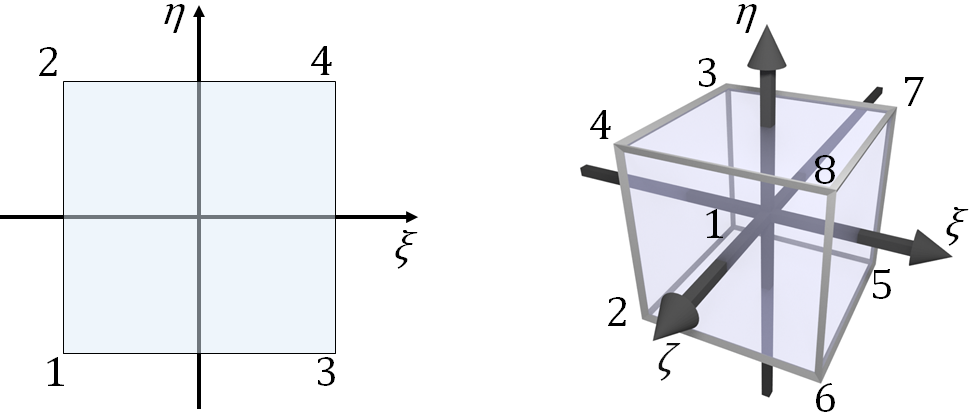
\includegraphics[width=0.8\textwidth]{figs/refEle.png}
\caption{Standard elements for 2D quadrilateral (left) 
	and 3D hexahedral elements (right). The standard element spans $[-1,1]$ in each axis
	to facilitate Gaussian quadrature rules. Nodes are marked with their indices.
	}
\label{fig:standardEle}
\end{figure}
\begin{table}
	\begin{center}
		\begin{tabular}{ |c| r r r|}
			\hline
			Index & $\xi_i$ & $\eta_i$ & $\zeta_i$ \\ \hline
			1 & -1 & -1 & -1\\  
			2 & -1 & -1 & 1\\
			3 & -1 & 1 & -1\\  
			4 & -1 & 1 & 1\\
			5 & 1 & -1 & -1\\  
			6 & 1 & -1 & 1\\
			7 & 1 & 1 & -1\\  
			8 & 1 & 1 & 1\\
		\hline						
		\end{tabular}
	\end{center}
	\caption{Nodal positions of the standard hexahedron element in the natural coordinates.
		Coincidentally, these coordinate values can also be used to define the trilinear interpolation weights.}
	\label{tab:natCoord}
\end{table}

With the interpolation function fully defined in the natural coordinates, 
we can use it to map a point $\chi$ in natural coordinates to a point
$\mathbf{X}$ inside a general hexahedron element with nodal positions $\mathbf{X}_i$ as follows
\begin{equation}
	\mathbf{X}=\sum_i N_i(\chi)\mathbf{X}_i.
	\label{eq:rest}
\end{equation}

Note here we are interpolating a vector-valued function where each coordinate is interpolated independently.
\subsection{Modeling Elastic Objects}
Elastic objects tend to return to its rest shape when deformed by external forces such as stretching, bending, twisting etc. The direction and strength of the tendency to restore to its rest shape is described by its elastic forces.
To model the exact behavior of a small piece of material,
we first use finite elements to approximate its deformations.
A hexahedron element models a piece of elastic material that can deform by changing its nodal positions.
The internal volume deforms by following the nodal displacements using trilinear interpolation.
Of course real materials do not have to deform this way.
The trilinear interpolation is only an approximation.
More precisely, for an element with a rest configuration given by $\mathbf{X}_i$,
its nodes can be moved to new positions $\mathbf{x}_i$ by displacements $\mathbf{u}_i$,
i.e., $\mathbf{x}_i=\mathbf{X}_i+\mathbf{u}_i$.
For any point $\mathbf{X}$ inside the element with known natural coordinates $\chi$, its displacement $\mathbf{u}(\mathbf{X})$ is given by interpolation
\begin{equation}
\mathbf{u}(\mathbf{X}) = \sum_iN_i(\chi)\mathbf{u}_i.
\label{eq:disp}
\end{equation}
From now on, to simplify notation, $N_i(\xi)$ will be written as $N_i$.
The deformation of an object is quantified using strain measures,
which is defined in terms of the difference in displacement between nearby points.
Intuitively, if $\mathbf{u}(\mathbf{X})$ is constant, then the displacement field is just a translation. In this case the material is undeformed and should not contain any strain.
More generally, the difference of displacement between nearby points can be written using derivatives,
\[
\mathbf{F}=\frac{\partial \mathbf{u}}{\partial \mathbf{X}}+\mathbf{I}
=\begin{pmatrix}
\dfrac{\partial u_1}{\partial X_1} & \dfrac{\partial u_1}{\partial X_2}&\dfrac{\partial u_1}{\partial X_3}\\
\dfrac{\partial u_2}{\partial X_1} & \dfrac{\partial u_2}{\partial X_2}&\dfrac{\partial u_2}{\partial X_3}\\
\dfrac{\partial u_3}{\partial X_1} & \dfrac{\partial u_3}{\partial X_2}&\dfrac{\partial u_3}{\partial X_3}\\
\end{pmatrix}+\mathbf{I}.
\]
The matrix $\mathbf{F}$ is the deformation gradient and $\mathbf{I}$ is the identity matrix.
While we do not have a closed-form expression of $\mathbf{u}$ written in terms of $\mathbf{X}$,
we have Equation~\ref{eq:rest} and~\ref{eq:disp} that relate $\mathbf{u}$ and $\mathbf{X}$ through $\chi$.
The term $\frac{\partial \mathbf{u}}{\partial \mathbf{X}}$ can be re-written using the chain rule,
\[
\frac{\partial \mathbf{u}}{\partial \mathbf{X}}=
\frac{\partial \mathbf{u}}{\partial \chi}
\frac{\partial \chi}{\partial \mathbf{X}}=
(\sum_i\mathbf{u}_i\frac{dN_i}{d\chi})(\frac{\partial \mathbf{X}}{\partial \chi})^{-1}
\]
The matrix $\frac{\partial \mathbf{X}}{\partial \chi}$ is called the Jacobian matrix of $\mathbf{X}$ with respect to $\chi$ and is written as
\[
\mathbf{J}=\frac{\partial \mathbf{X}}{\partial \chi}
= \sum_i\mathbf{X}_i\frac{dN_i}{d\chi}.
\]
By convention, $\frac{dN_i}{d\chi}$ is a $1\times 3$ row vector.
The term $\mathbf{X}_i\frac{dN_i}{d\chi}$ is an outer product that produces a $3\times 3$ matrix.

\section{}
